%% =====================================================================
%%  Temporally Constrained, Provenance-Verified Evidence Retrieval
%%  for Indian Legal Research
%%
%%  IEEE conference format (IEEEtran). Compiles on Overleaf as-is:
%%  select "pdfLaTeX", place the figures/ directory alongside this file.
%% =====================================================================

\documentclass[conference]{IEEEtran}
\IEEEoverridecommandlockouts

\usepackage{cite}
\usepackage{amsmath,amssymb}
\usepackage{graphicx}
\usepackage{booktabs}
\usepackage{multirow}
\usepackage{url}
\usepackage{xurl}   % allow long URLs to break anywhere (repo link in Sec. Reproducibility)
\usepackage[hidelinks]{hyperref}
\usepackage{xcolor}

\def\BibTeX{{\rm B\kern-.05em{\sc i\kern-.025em b}\kern-.08em
    T\kern-.1667em\lower.7ex\hbox{E}\kern-.125emX}}

% Tighter tables in two-column layout
\renewcommand{\arraystretch}{1.12}

\begin{document}

\title{Temporally Constrained, Provenance-Verified\\
Evidence Retrieval for Indian Legal Research}

% ---------------------------------------------------------------------
% AUTHOR BLOCK -- replace placeholders before submission.
% ---------------------------------------------------------------------
\author{
% NOTE: do not wrap placeholders in square brackets on a line that follows
% "\\" -- LaTeX reads "\\[...]" as an optional vertical-space argument.
\IEEEauthorblockN{Yuvraj Singh (yuvraj.singh@akgec.ac.in)\\
RishiRaj Jaiswal (rishiraj.jaiswal@akgec.ac.in)\\
Rahul Ranjan (rahul.ranjan@akgec.ac.in)\\
Saurav Kumar Chaudhary (saurav.chaudhary@akgec.ac.in)}
\and
\IEEEauthorblockN{Kriti Mishra (Supervisor)}
\IEEEauthorblockA{\textit{Department of Computer Science and Engineering} \\
\textit{Ajay Kumar Garg Engineering College} \\
Ghaziabad, India \\
kriti.mishra@akgec.ac.in}
}

\maketitle

% =====================================================================
\begin{abstract}
AI-assisted legal research fails in ways that fluent output conceals: a cited
authority may not exist, may not contain the attributed passage, may post-date
the matter under analysis, or may never have been retrieved at all. A 2026
Supreme Court of India ruling overturned tribunal findings that had relied on
exactly these defects, turning citation verifiability from a matter of style
into a functional requirement for any such system. This paper presents an
evidence pipeline for
historical Indian Supreme Court judgments in which every displayed citation is
temporally eligible, provenance-bound, and mechanically verifiable against the
persisted corpus. The design is deliberately extractive: material propositions
are shown verbatim with page and character locators, and outcome prediction is
kept in a separate field so that a classification score can never stand in for
evidence quality. We report three findings on a combined 37-case
reference-evidence population (a frozen 30-case base plus a later additive
7-case verified extension, analysed in strata throughout). First, a
cross-corpus audit shows
that naive identifier matching between the ILDC corpus and an eCourts-derived
judgment archive is unsafe: of 5{,}391 syntactically matching identifiers only 11
survived content alignment, motivating a reusable content-alignment gate.
Second, moving temporal eligibility into the BM25 candidate relation
\emph{before} ranking, together with salient-term query construction and a
coverage-qualified self-match guard, raised expected-authority Recall@5 from
5/30 to 12/30 and Recall@100 from 12/30 to 15/30 on the frozen base; on the
combined 37 cases Recall@5 is 12/37 and Recall@100 is 20/37. Third, and
centrally, all 185 displayed citations passed grounding, provenance, and
temporal verification, with zero unsupported claims across the 37 cases,
while 17 of the 37 expected authorities remained
absent at $k{=}100$. Perfect verification of what a system displays is therefore
compatible with substantially incomplete retrieval, and the two must be measured
on separate denominators. Auxiliary outcome baselines on 1{,}503 held-out ILDC
cases and an inference-time evidence-augmentation extension are reported with
their own populations and stated limits. A blinded 14-case, four-LLM-rater
exploratory comparison favoured the structured presentation 56/56, which we
report as presentation evidence only, not human-subject evidence.
\end{abstract}

\begin{IEEEkeywords}
legal information retrieval, explainable AI, provenance verification, temporal
filtering, retrieval-augmented systems, Indian legal NLP, BM25, InLegalBERT
\end{IEEEkeywords}

% =====================================================================
\section{Introduction}

Legal research operates in a domain where fluency is not evidence. A generated
response can be linguistically convincing while citing a judgment that does not
exist, attributing a passage to a real judgment that does not contain it, or
relying on law that was unavailable at the time the matter arose. Empirical
profiling of legal hallucination in large language models has established that
these failures are frequent rather than exceptional \cite{dahl2024}, and related
work has probed how far explicit legal standards can be communicated to language
models at all \cite{nay2023}.

The problem is no longer confined to the literature. In \emph{Pooja Ramesh Singh
v.\ Jammu and Kashmir Bank Ltd.\ \& Anr.}, 2026 INSC 668, the Supreme Court of
India set aside tribunal decisions after identifying nonexistent authorities,
incorrect citations, and fabricated passages apparently produced through
AI-assisted research \cite{poojasingh2026}. The Court distinguished legitimate
assistance from unverified reliance and emphasised continued human control over
adjudication. The judgment converts an accuracy concern into a systems
requirement: a legal research tool must produce evidence that a reviewer can
locate, inspect, and independently verify, not merely an answer that reads as
legal.

This paper treats that requirement as the primary design constraint. We build
and evaluate an evidence pipeline over historical Indian Supreme Court
judgments in which the answer layer is extractive by construction. Given facts
extracted from a query judgment, the system retrieves earlier Supreme Court
material, retains stable source and passage locators through every stage,
excludes the query judgment and its content-aligned duplicates, renders only
selected verbatim passages, and then verifies each displayed citation against
the persisted corpus and the recorded retrieval run. Outcome prediction is
available but structurally subordinated: it is emitted in a separate top-level
field and never alters the evidence-bound conclusion.

The central empirical observation is a dissociation that a single aggregate
score would erase. Under the final configuration, all 185 displayed citations
across the combined 37 cases
cleared grounding, provenance, duplicate, and temporal checks, with no
unsupported claim among the 37 cases; at the same time, 17 of the 37 independently
verified expected authorities never appeared among the top 100 candidates
returned by the retriever. Correctness of what is shown and completeness of
what is found are therefore separate properties, and a system can score
perfectly on the first while still missing outcome-relevant material on the
second. Reporting only a combined ``citation correctness'' figure would hide
exactly the gap a reader needs in order to decide how much to trust the
output.

\textbf{Contributions.} This work makes four contributions, each bounded to the
evaluated setting.

\begin{enumerate}
\item \textbf{A quantified cross-corpus identity failure and its remedy.}
Converting eCourts identifiers of the form \texttt{YYYY INSC N} to ILDC-style
\texttt{YYYY\_N} produced 5{,}391 syntactic candidates, of which only 11 passed
content alignment (Section~\ref{sec:alignment}). We show that identifier
equality is unsafe for this widely used dataset pair and supply a reusable
content-alignment gate based on title/party identity plus direct phrase overlap.

\item \textbf{Pre-ranking temporal eligibility.} We implement historical
availability as a predicate inside the BM25 candidate relation rather than as a
post-hoc filter, so that ineligible judgments cannot consume retrieval depth
(Section~\ref{sec:e3}). On the held-out evidence set this change moved
Recall@5 from 5/30 to 12/30 without regressing any prior success.

\item \textbf{A four-state citation protocol with separate denominators.} We
distinguish fabricated citations, real-but-unretrieved citations, retrieved
citations violating policy, and valid citations that simply differ from the
reference authority (Section~\ref{sec:protocol}) --- four states that a single
correctness label collapses.

\item \textbf{An evaluation that keeps recovery and integrity apart.} We report
authority recovery, citation integrity, outcome prediction, and explanation
presentation on their own populations, and document the resulting dissociation
rather than resolving it into a headline number (Section~\ref{sec:results}).
\end{enumerate}

\textbf{Scope.} The claims are deliberately narrow. We do not establish legal
correctness for retrieved authorities, deploy an autonomous legal advisor, or
show that evidence retrieval improves outcome prediction. The system is a
researcher-facing prototype evaluated on four distinct and non-pooled
populations: 1{,}503 outcome cases, 30 frozen plus 7 additive source-verified
evidence cases analysed in strata, and paired explanation examples (seven
formative author-reviewed pairs, superseded by a 14-case exploratory LLM
comparison).

% =====================================================================
\section{Related Work}

\subsection{Indian legal NLP and judgment prediction}

The ILDC corpus established Indian Supreme Court judgment prediction and
explanation as a benchmark task \cite{malik2021}, and supplies the fixed splits
and binary outcome labels used for the baselines here. Domain-adapted
pre-training for Indian law produced InLegalBERT and related models
\cite{paul2023}, which motivate our neural baseline. Work on long Indian
judgment summarisation with practitioner evaluation \cite{shukla2022}
established that document length and expert-facing presentation are first-order
concerns in this jurisdiction. None of these lines addresses cross-corpus source
identity or per-citation provenance, which is where this work sits.

\subsection{Legal retrieval, entailment, and benchmarks}

COLIEE evaluates case-law and statute retrieval and entailment \cite{coliee2023};
LegalBench measures multiple forms of legal reasoning in large language models
\cite{legalbench2023}; CaseHOLD tests selection of cited-case holdings and the
value of legal-domain pre-training \cite{casehold2021}. These benchmarks set a useful bar for retrieval quality and evaluation
rigor, but each operates over one fixed, curated corpus and none requires a
candidate to have existed, or been decided, before the query matter arose.

\subsection{Temporal and provenance constraints}

TaxFlow applies hybrid RAG with temporal filtering to Indian statutory tax
question answering \cite{taxflow2026}, sharing our concern that legal retrieval
must respect changing law. CaseFacts frames U.S.\ legal claim verification with
Supported/Refuted/Overruled labels \cite{casefacts2026}, demonstrating that
legal validity evolves. LexTime benchmarks temporal ordering of events in U.S.\
federal complaints \cite{lextime2025}. Retrieval-augmented generation
established retrieval as an explicit non-parametric evidence source
\cite{lewis2020}; BM25 supplies the sparse ranking basis \cite{robertson2009}
and Tesseract the OCR engine for corpus repair \cite{smith2007}.

\subsection{Positioning}

Table~\ref{tab:related} states the boundary of the present contribution against
the closest work. We claim neither the first legal RAG system, nor the first
Indian legal model, nor the first temporal legal benchmark. The contribution is
the reproducible combination of cross-corpus content-alignment gating,
conservative pre-ranking eligibility, exact passage and retrieval-run
verification, and separate reporting of authority recovery versus citation
validity against a source-first answer key. Because jurisdictions, tasks,
corpora, and denominators differ across these systems, none is used as a
directly comparable numerical baseline; we compare only experiments run under
our own frozen populations.

\begin{table*}[t]
\caption{Positioning against the closest related work. No external system is
used as a numerical baseline, because jurisdictions, tasks, corpora, and
denominators differ.}
\label{tab:related}
\centering
\small
\begin{tabular}{p{2.1cm}p{4.6cm}p{4.4cm}p{5.2cm}}
\toprule
\textbf{Work} & \textbf{Task and setting} & \textbf{Relation to this work} &
\textbf{Boundary of present contribution} \\
\midrule
ILDC / CJPE \cite{malik2021} &
Indian Supreme Court outcome prediction and explanation &
Supplies the prediction setting and the fixed ILDC Single splits &
We use a fixed ILDC subset for baselines and add a separate, provenance-bearing
evidence corpus; we do not reproduce the CJPE architecture \\
\addlinespace
InLegalBERT \cite{paul2023} &
Domain-adapted pre-training for Indian legal tasks &
Motivates the pinned neural outcome baseline &
We correct long-document truncation via chunk-and-pool and do not assume domain
pre-training must beat a sparse baseline \\
\addlinespace
TaxFlow \cite{taxflow2026} &
Hybrid RAG with temporal filtering for Indian statutory tax QA &
Shares the premise that legal retrieval must respect changing law &
We address historical precedent retrieval, cross-corpus identity, exact
displayed-passage provenance, and a source-verified authority key \\
\addlinespace
CaseFacts \cite{casefacts2026} &
U.S.\ legal claim verification and precedent retrieval &
Shows legal validity evolves and unrestricted retrieval admits noisy sources &
We query from historical Indian case facts and verify source identity, temporal
eligibility, and retrieval provenance rather than claim labels \\
\addlinespace
LexTime \cite{lextime2025} &
Temporal ordering of events in U.S.\ federal complaints &
Establishes temporal reasoning as a distinct legal-language challenge &
Our task is not event ordering; we enforce historical availability through
metadata before ranking \\
\bottomrule
\end{tabular}
\end{table*}

% =====================================================================
\section{Problem Formulation}
\label{sec:problem}

Let a historical query judgment have identifier $q$, query year $Y_q$, and
frozen facts-only text $F_q$. Let each candidate evidence passage $p$ belong to
a source judgment with a stable source identifier, an exact decision date,
citation metadata, page and character boundaries, and stored passage text.

The temporal policy admits $p$ only when the decision year of its source is
strictly earlier than $Y_q$. A same-year source is treated as ambiguous, because
ILDC supplies no exact query date; a source with missing or unparseable date
metadata is excluded. Both rules are deliberately conservative: they trade
recall for the guarantee that no displayed authority can post-date the matter.

The evidence task decomposes into three separable questions.

\begin{itemize}
\item \textbf{Recovery.} Does the top-100 candidate set contain the
independently verified expected authority, and is that authority among the five
displayed sources?
\item \textbf{Integrity.} Does each displayed citation reproduce a real
retrieved corpus passage with exact provenance, avoid the query judgment and its
aligned duplicates, and satisfy the temporal rule?
\item \textbf{Presentation.} Given identical evidence and citations, does a
structured Issue--Authority--Evidence--Conclusion--Uncertainty format make the
material easier to inspect than unstructured prose?
\end{itemize}

Outcome prediction is a secondary evaluation capability, not a fourth research
question. It is reported on its own
population and never pooled with the evidence measures, so that a classification
score cannot substitute for evidence quality and a traceable citation cannot be
mistaken for complete authority recovery. Table~\ref{tab:defs} fixes the
operational definitions and pass/fail criteria.

\subsection{Research questions}

There are exactly three research questions. \textbf{RQ1:} Does grounding an
Indian legal AI workflow in retrieved legal evidence improve legal-research
reliability and relevant-evidence retrieval compared with a facts-only
legal-language baseline? The controlled comparison is E2 versus E3; E1 is a
traditional baseline reported for context. \textbf{RQ2:} Does
provenance-constrained evidence selection and citation verification reduce
unsupported or unverifiable legal claims in the final output?
\textbf{RQ3:} Can the proposed structured explanation format improve
human-verifiable transparency without materially degrading prediction or
retrieval performance?

\begin{table}[t]
\caption{Operational definitions used throughout the frozen evaluation.}
\label{tab:defs}
\centering
\footnotesize
\begin{tabular}{p{2.35cm}p{5.5cm}}
\toprule
\textbf{Term} & \textbf{Implemented definition} \\
\midrule
Facts-only input &
Text retained before the earlier of a recognised dispositive cue and a 60\%
character cap, sentence-aligned where possible; inputs below 10\% retention or
100 words are excluded \\
\addlinespace
Temporal existence &
The source has a parseable exact decision date in corpus metadata \\
\addlinespace
Temporal applicability &
For query year $Y$, an authority is eligible only if its decision year is
$< Y$; same-year, later-year, and missing-date sources are excluded \\
\addlinespace
Temporal effectiveness &
The eligibility predicate is applied inside the BM25 candidate relation before
ranking and \texttt{LIMIT 100}, so ineligible sources cannot consume returned
depth \\
\addlinespace
Recall@100 &
Share of answer-key cases whose predefined authority occurs anywhere in the
returned top-100 candidates \\
\addlinespace
Recall@5 &
Share of answer-key cases whose predefined authority is among the five selected
and displayed sources \\
\addlinespace
Provenance validity &
A displayed item reproduces the stored source ID, citation, decision date,
court, PDF/page/character locator, exact passage, and retrieval-run membership \\
\addlinespace
Citation groundedness &
Every material displayed proposition is verbatim text of a supplied evidence
passage and links to that evidence item \\
\addlinespace
Authority consistency &
A verified displayed source matches the answer-key authority by stable source
ID, normalised citation, or normalised title plus exact decision date \\
\bottomrule
\end{tabular}
\end{table}

% =====================================================================
\section{Corpus Construction and Auditing}

\subsection{Purpose-split corpus design}

We use two corpora for different experimental purposes rather than treating
them as interchangeable records of the same judgments.

ILDC Single supplies fixed case-level splits and binary outcome labels. The
local release contains 7{,}593 judgments: 5{,}082 training, 994 validation, and
1{,}517 test cases. After a shared sufficiency rule excluded 14 test records,
the held-out prediction population contains 1{,}503 cases.

The evidence corpus is an eCourts-derived collection of Indian Supreme Court
judgments covering 1950--2020, providing judgment PDFs and the metadata absent
from ILDC: citations, exact decision dates, court and case identifiers, source
paths, and page and character locators. The download contained 39{,}069 English
PDF instances. After quality repair and exclusion, 39{,}066 PDFs yielded
2{,}343{,}435 labelled chunks, of which 2{,}036{,}981 unique chunks were loaded
into a PostgreSQL provenance store and a SQLite FTS5 BM25 index.

This split follows the information actually available in each source. ILDC
supports fixed-split outcome prediction but exposes only a year in the case
identifier and lacks the citation and passage provenance that verification
requires. The eCourts collection supports dated, traceable retrieval but is not
used as a substitute outcome-label benchmark. Cross-corpus links are drawn only
after the alignment checks described below.

\subsection{Source-quality audit and targeted OCR repair}

A full audit found the stored text valid UTF-8, but 15 PDF instances
(representing 14 source IDs) had missing or badly corrupted embedded text.
Failures concentrated in image-backed Supreme Court Reports from the 1980s and
1990s, with one mojibake-affected 2018 file. Fixed checks covered absent
embedded text, control characters, mojibake markers, visible-ASCII ratio, and
English-token ratio.

Only flagged instances were re-rendered and processed with English Tesseract OCR
at 250\,DPI \cite{smith2007}. Twelve passed the same post-OCR quality gate and
were restored; three single-page PDFs remained below threshold and were
transparently excluded rather than forced into the index. Raw PDFs were
preserved unchanged, exclusions were recorded, and the provenance store and BM25
index were rebuilt from the accepted corpus.

\subsection{Cross-corpus identifier alignment}
\label{sec:alignment}

Linking ILDC query cases to eCourts sources requires establishing that two
records describe the same judgment. The obvious route --- converting an eCourts
identifier of the form \texttt{YYYY INSC N} to the ILDC-like string
\texttt{YYYY\_N} --- is unsafe, and quantifiably so.

That conversion produced 5{,}391 syntactic candidates. \textbf{Only 11 passed
content alignment; 5{,}380 were identifier-namespace collisions.} The failure is
not a single offset or an isolated scrape defect: it concentrates in legacy
material where similar numeric suffixes routinely denote entirely different
judgments. A pipeline that trusts identifier equality here would silently merge
unrelated cases, corrupting both deduplication and leakage control.

The corrected pipeline treats identifier equality as candidate generation only.
A reusable gate evaluates title or party identity together with direct six-token
phrase overlap before any mapping may drive deduplication or retrieval
exclusion. Combining syntactic and title/party candidates yielded 8{,}927
deduplicated pairs, of which 1{,}304 were accepted and 7{,}623 rejected.
Retrieval additionally applies a full-document self-match safeguard, so that an
unmapped copy of the query judgment can be removed without suppressing an
earlier authority merely quoted at length by the later judgment.

We regard this audit as independently useful. It demonstrates that mechanically
similar ILDC and eCourts identifiers do not establish judgment identity, and it
supplies a content-based alternative reusable across answer-key validation,
development probes, leakage checks, and retrieval-time exclusion.

\subsection{Source-verified authority answer key}

The authority evaluation uses 30 ILDC fixed-test cases. Test membership was
confirmed before external verification. For each accepted case the query
judgment was inspected through a primary source or accepted eCourts mirror, one
earlier authority was recorded \emph{independently of system retrieval}, and
that authority was reconciled to the corpus by stable source ID, normalised
citation, or normalised title plus exact date for parallel reporter forms.

The identifier-collision discovery triggered a read-only audit of the
then-current mappings: 20 passed, nine resolved sources failed direct content
alignment, and one source was unresolved. One case was relinked to a
content-aligned source and the other nine flagged records were replaced by new
fixed-test cases, yielding a final audit of 30/30 direct-content passes.

The sample is not era-balanced: five query cases are from the 1970s, 13 from the
1980s, nine from the 1990s, two from the 2000s, and one from the 2010s. The
1980s account for 43.3\%. This concentration is a consequence of the source and
alignment gates rather than deliberate temporal sampling, and we treat it as a
limitation (Section~\ref{sec:limits}).

A later additive extension verified seven further fixed-test cases under the
same gates, without modifying the original 30-case key: \texttt{1990\_234},
\texttt{1990\_256}, \texttt{1990\_324}, \texttt{1991\_136},
\texttt{1991\_87}, \texttt{1992\_286}, \texttt{1993\_90}. Three further
candidates were held back as needing review (a background listing, an
unresolved court treatment, and a party-only reliance) and are not part of
any evaluation. The combined 37-case population is therefore a later expanded
analysis, not the preregistered frozen base; all results below retain
Base-30, Extension-7, and Combined-37 strata so the original 30-case
evaluation remains independently reproducible.

% =====================================================================
\section{System Design}

The system comprises four auditable layers.

\textbf{1. Corpus and alignment layer.} ILDC split files supply prediction cases
and labels. Cleaned eCourts chunks retain stable source, date, citation, court,
PDF, page, and character provenance. A content-aligned crosswalk plus a runtime
content check control target-case leakage.

\textbf{2. Outcome branch.} A shared facts-only extractor feeds a sparse linear
baseline (E1) and an InLegalBERT chunk-and-pool model (E2). These baselines
produce binary predictions and never retrieve external evidence.

\textbf{3. Evidence branch (E3).} Full facts-only text is converted to salient
terms, matched through BM25 under pre-ranking temporal eligibility, and narrowed
to five source-diverse passages. The renderer emits these passages in a fixed
evidence-linked structure.

\textbf{4. Verification and reporting layer (E4).} Each displayed evidence
record is verified against the corpus and the recorded retrieval run; duplicate
and temporal rules are enforced; verified sources are then separately compared
with the source-first answer key. Versioned JSON and Markdown artifacts preserve
metrics, failures, and configuration provenance.

The answer layer is deliberately extractive. It favours inspectability over
fluent synthesis: material legal text is displayed verbatim, and the conclusion
is fixed, non-inferential wording tied to evidence identifiers. The renderer
cannot retrieve, rerank, invent an authority, paraphrase a material proposition,
or infer an outcome.

% =====================================================================
\section{Method}

\subsection{Shared facts-only input}

E1 and E2 share the extraction configuration \texttt{ildc-predecision-facts-v1}.
The extractor retains text preceding the earlier of a recognised dispositive cue
and 60\% of the document, moving the boundary to a preceding sentence end when
sufficient text remains. Cases below 10\% retention or 100 words are excluded.
Neither prediction path uses retrieval. Model and threshold selection uses
validation data only; the held-out test split is evaluated once, after
selection.

\subsection{E1: sparse linear baseline}

E1 uses lowercased, Unicode-normalised TF--IDF unigrams and bigrams with
sublinear term frequency, minimum document frequency two, $L_2$ normalisation,
and at most 100{,}000 features. Logistic-regression values
$C \in \{0.1, 1.0, 10.0\}$ are compared by validation accuracy, with smaller $C$
breaking ties. The selected $C = 10.0$ pipeline is refitted once on eligible
training and validation cases and evaluated once on test data. Seed 202605.

\subsection{E2: InLegalBERT chunk-and-pool}

E2 fine-tunes \texttt{law-ai/InLegalBERT} (revision
\texttt{b5ecfed8}) with a new two-label head. It supersedes an
earlier 256-token prefix run that truncated 99.20\% of eligible test inputs ---
a discarded result we retain for traceability. Each facts-only document is
instead represented by overlapping 512-token windows with 50-token overlap.
Training uses three epochs, seed 202607, learning rate $2\times10^{-5}$, weight
decay 0.01, warm-up ratio 0.1, gradient checkpointing, and gradient
accumulation.

Mean pooling of window logits before softmax is the primary rule, and checkpoint
selection uses validation document-level mean-logit accuracy only. Majority vote
is reported as a secondary comparison, not a post-hoc selection rule. All
1{,}503 eligible test documents and 9{,}576 test windows are covered.

\subsection{E3: temporally constrained retrieval}
\label{sec:e3}

The query builder \texttt{tfidf-segment-salient-terms-v1} segments the full
facts-only input, removes procedural-report boilerplate, scores terms
deterministically, retains section and article cues, and emits at most 32 unique
terms. These query a SQLite FTS5 BM25 index backed by PostgreSQL provenance.

The frozen configuration is
\texttt{week11-bm25-salient-terms-preranked-temporal-v3}. The critical design
choice is placement: only judgments with decision year strictly earlier than the
query year enter the candidate relation \emph{before} BM25 ordering and the
top-100 cutoff. Applied afterwards, the same rule would allow ineligible
judgments to occupy returned depth and be discarded, shrinking the effective
candidate pool; applied before, the full depth is spent on eligible material.

Candidate sources are checked against the alignment-gated crosswalk and a direct
self-match rule requiring at least 100 shared six-token occurrences and 80\%
unique candidate-source phrase coverage. A non-learned selector then chooses up
to five passages in BM25 order, with at most one passage per source.

\subsection{E4: citation and provenance verification}

E4 receives the E3 answer, the retrieval-run identifier, query identity and
year, and the persisted corpus records. Each displayed item must exist in the
corpus, reproduce its exact passage and provenance, belong to the recorded
retrieval run, avoid the query and its aligned duplicates, and pre-date the
query year. Any failure rejects the citation.

Authority consistency is evaluated separately, after verification. A fully valid
citation may differ from the single expected authority without being labelled
substantively irrelevant --- a distinction we return to in
Section~\ref{sec:ceiling}.

\subsection{Inference-time evidence augmentation}

Outcome prediction was subsequently added to E3 and E4 by reusing the frozen E2
checkpoint without fine-tuning. A shared input builder concatenates the frozen
facts extract and the selected verbatim evidence in selection order, applies the
same 512-token windows with 50-token overlap, pools window logits by their mean,
and selects the class by \texttt{argmax}. Labels, citation identifiers,
retrieval scores, decision dates, provenance fields, and rendered boilerplate
are excluded from model input. Seed 202607; configuration
\texttt{e3e4-evidence-augmented-inlegalbert-checkpoint6318-v1}.

We note the methodological caveat plainly: the checkpoint was trained on
facts-only inputs, so applying it to facts plus retrieved passages is an
inference-time distribution shift, not evidence-aware fine-tuning. These
predictions are therefore reported descriptively --- on the frozen 30-case
base and, in the RQ1 extension, on the combined 37 cases --- and are
not directly comparable with the 1{,}503-case baselines, which form a
separate population with a different denominator.

\subsection{Bundled-intervention caveat}

E4 is not a single-variable ablation of E3. It jointly checks corpus existence,
exact passage and provenance identity, retrieval-run membership, duplicate
status, and temporal eligibility, and both stages share the same final retrieval
and selected evidence. Aggregate reliability cannot be attributed to any one
verification component; the supported claim concerns the complete bundle.

% =====================================================================
\section{Citation and Provenance Protocol}
\label{sec:protocol}

Each chunk in the corpus is keyed by a stable identifier built from where it
originated (source path) and where it sits within that source (passage
location). Against that key, the persisted record stores: source ID, source
case ID where available, citation, exact decision date, court, local PDF
file, page number, character start and end, and chunk text. Retrieval runs record query ID, year,
query text, index version, temporal policy, rank, score, and temporal status.

The renderer may expose only supplied selected evidence. Material content
remains verbatim; authority cards and conclusions refer to evidence IDs.
Verification then checks corpus existence, exact field equality, run membership,
duplicate status, and temporal eligibility. Answer-key matching occurs only
after a displayed citation has passed these checks. Parallel reporter forms are
reconciled through stable source identity or normalised title plus exact
decision date, never loose string similarity.

This protocol distinguishes four failure states that a single
``correct citation'' label would collapse:

\begin{enumerate}
\item a fabricated or altered citation;
\item a real citation that was not retrieved for this query;
\item a retrieved citation violating temporal or duplicate policy;
\item a fully valid citation that does not match the predefined expected
authority.
\end{enumerate}

Keeping these separate is what allows failures to be located rather than merely
counted. In our results, states (1)--(3) occur zero times and state (4) occurs
in 18 of 30 cases --- a profile that a single aggregate score would render
invisible.

% =====================================================================
\section{Results}
\label{sec:results}

\subsection{Reporting populations}

Four populations are reported and never aggregated across kinds: 1{,}503 eligible fixed
ILDC test cases for outcome prediction; a combined 37-case reference-evidence
population for authority recovery, evidence-augmented prediction, and 185
displayed-citation verifications, always stratified as Base-30 (the frozen
key: 150 citations), Extension-7 (the additive verified cases: 35
citations), and Combined-37; and paired cases for explanation-format review
(seven formative author-reviewed pairs, superseded as the principal RQ3
result by the 14-case LLM exploratory evaluation below).

\subsection{Outcome prediction}

Table~\ref{tab:outcome} reports the outcome results. On the 1{,}503-case
population, the sparse E1 baseline reached accuracy 0.6134 and macro-F1 0.6123,
exceeding corrected E2 mean-logit pooling at 0.5968 and 0.5924. E2's secondary
majority-vote aggregation reached 0.6015 and 0.5937. All primary models exceeded
the 0.5017 majority-class accuracy.

\begin{table}[t]
\caption{Outcome prediction. Populations are distinct and must not be compared
as a like-for-like leaderboard.}
\label{tab:outcome}
\centering
\footnotesize
\setlength{\tabcolsep}{4pt}
\begin{tabular}{lccc}
\toprule
\textbf{Model} & \textbf{$n$} & \textbf{Acc.} & \textbf{Macro-F1} \\
\midrule
Majority class            & 1{,}503 & 0.5017 & 0.3341 \\
E1 TF--IDF + LR           & 1{,}503 & \textbf{0.6134} & \textbf{0.6123} \\
E2 InLegalBERT, mean logits & 1{,}503 & 0.5968 & 0.5924 \\
E2 InLegalBERT, maj.\ vote  & 1{,}503 & 0.6015 & 0.5937 \\
\midrule
E3 evidence-augmented     & 30 & 0.6667 & 0.6032 \\
E4 verified evid.-augmented & 30 & 0.6667 & 0.6032 \\
\bottomrule
\end{tabular}
\end{table}

\begin{figure}[t]
\centering
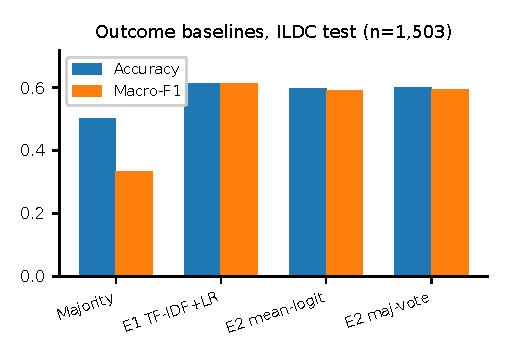
\includegraphics[width=\columnwidth]{figures/fig1_outcome.pdf}
\caption{Accuracy and macro-F1 for E1, corrected E2 under both pooling rules,
and the majority baseline on the eligible ILDC test population ($n=1{,}503$).}
\label{fig:outcome}
\end{figure}

This result does not show that domain pre-training is ineffective in general. It
shows that under the implemented facts extraction, data size, training budget,
window aggregation, and frozen settings, the sparse baseline performed better.
The per-case analysis in Section~\ref{sec:error} shows the two models make
substantially non-identical errors.

On the separate 30-case subset, evidence-augmented E3 and verified E4 both
reached accuracy 0.6667 and macro-F1 0.6032, with identical confusion matrices.
On the combined 37 cases the same shared predictor reaches accuracy 0.6486 and
macro-F1 0.6073 with confusion matrix [[6,3],[10,18]], again identical for E3
and E4 (Table~\ref{tab:rq1strata}).
\textbf{The equality is expected and is not evidence that verification is
redundant.} E4 verification did not reject any evidence in this run, so the
predictor received an identical input; E4's contribution is control,
traceability, and explanation, not a different decision rule. A configuration in
which verification rejected evidence would produce differing scores, and the
architecture reports both so that such a divergence would be visible.

\subsection{Authority recovery and evidence integrity}

On the 30-case answer-key subset, expected-authority Recall@5 was 0.40 (12/30)
and Recall@100 was 0.50 (12 selected $+$ 3 retrieved-but-unselected $=$ 15/30
found within $k{=}100$). The remaining 15 authorities were absent at $k{=}100$.

The principal RQ1 result uses the combined 37-case population
(Table~\ref{tab:rq1strata}). The seven extension cases contribute no
additional top-5 recovery (0/7) but five further top-100 recoveries at ranks
14, 16, 26, 32, and 89, with two absent; their displayed citations are
likewise fully verified (35/35). The combined figures are therefore Recall@5
12/37 $=$ 0.324324 and Recall@100 20/37 $=$ 0.540541 over 185 displayed
citations. The lower combined Recall@5 is descriptive of the added stratum,
not evidence about the base configuration, and the frozen 30-case result
above is retained unchanged alongside it.

\begin{table}[t]
\caption{RQ1 retrieval and evidence-augmented prediction by stratum. The
combined row is the principal evaluation; strata are never pooled silently.}
\label{tab:rq1strata}
\centering
\footnotesize
\setlength{\tabcolsep}{4pt}
\begin{tabular}{lrrrrr}
\toprule
\textbf{Population} & \textbf{$n$} & \textbf{R@5} & \textbf{R@100} &
\textbf{E3 Acc.} & \textbf{E3 Macro-F1} \\
\midrule
Base-30          & 30 & 0.40 (12/30) & 0.50 (15/30)   & 0.6667 & 0.6032 \\
Extension-7      & 7  & 0.00 (0/7)   & 0.7143 (5/7)   & 0.5714 & 0.5714 \\
Combined-37      & 37 & 0.3243 (12/37) & 0.5405 (20/37) & 0.6486 & 0.6073 \\
\bottomrule
\end{tabular}
\end{table}

Figure~\ref{fig:funnel} shows the recovery funnel.

All 150 displayed citations were grounded, provenance-valid, and temporally
eligible, with zero unsupported claims across the 30 cases (Table~\ref{tab:integrity},
Figure~\ref{fig:integrity}). The final candidate log contained 3{,}000/3{,}000
eligible candidates. In a five-case explanation-faithfulness check, every
evidence reference resolved to the exact persisted retrieved chunk. Over the
combined 37 cases the same profile holds at larger denominators: 185/185
grounded and provenance-valid, 0/185 temporal violations, 0/37 unsupported
claims.

E4 verification is fail-closed: any failing check rejects the citation and
no verified output is produced for that case. On live data no citation was
rejected, which is a ceiling effect of already-valid selected evidence, not
a measure of the gate's strength. Three positive controls through the
unchanged verifier demonstrate that strength directly: altered verbatim
passages were rejected 37/37, fabricated authority citations 37/37, and
backdated query years rendering authorities ineligible 37/37.

\begin{table}[t]
\caption{Evidence recovery and integrity on the frozen Base-30 answer-key
stratum ($n=30$
queries; 150 displayed citations). Combined-37 values are reported in
Table~\ref{tab:rq1strata} and the surrounding text.}
\label{tab:integrity}
\centering
\footnotesize
\setlength{\tabcolsep}{4pt}
\begin{tabular}{lcl}
\toprule
\textbf{Measure} & \textbf{Value} & \textbf{Arithmetic} \\
\midrule
Recall@5            & 0.40 & 12 of 30 in top 5 \\
Recall@100          & 0.50 & 15 of 30 in top 100 \\
Absent at $k{=}100$ & 0.50 & 15 of 30 \\
Authority precision & 0.08 & 12 of 150 shown \\
\quad struct.\ ceiling & 0.20 & 30 of 150 (5 shown, 1 credited) \\
Grounding           & 1.00 & 150/150 passed \\
Provenance validity & 1.00 & 150/150 passed \\
Temporal violations & 0    & 0 of 150 \\
Unsupported claims  & 0    & 0 of 30 cases \\
\bottomrule
\end{tabular}
\end{table}

\begin{figure}[t]
\centering
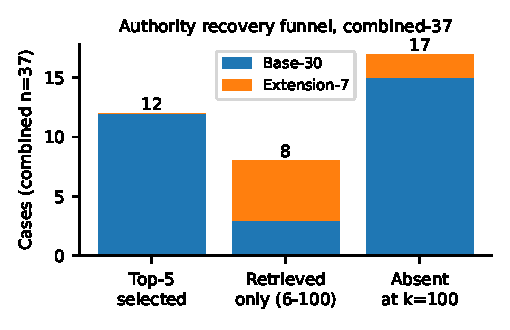
\includegraphics[width=\columnwidth]{figures/fig2_funnel.pdf}
\caption{Expected-authority recovery on the combined reference set
($n=37$): 12 retrieved and selected, eight retrieved but unselected (three
base, five extension), and 17 absent at $k{=}100$.}
\label{fig:funnel}
\end{figure}

\begin{figure}[t]
\centering
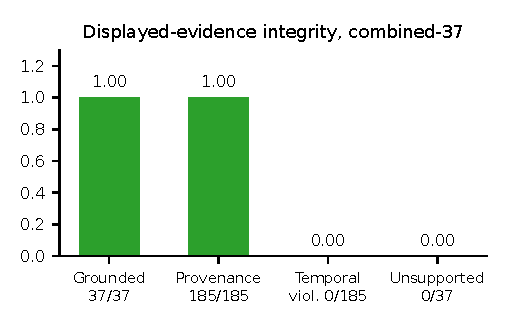
\includegraphics[width=\columnwidth]{figures/fig3_integrity.pdf}
\caption{Displayed-evidence integrity under the final configuration
(combined $n=37$ queries; 185 displayed citations): all grounding and
provenance checks passed,
with no temporal violations or unsupported claims. The frozen Base-30
stratum contributes 150/150 of these checks.}
\label{fig:integrity}
\end{figure}

\textbf{This is the paper's central result.} Verification success and authority
recovery are dissociated: the system verified everything it displayed (185/185
combined; 150/150 on the frozen base) while recovering the expected authority
in 20 of 37 cases at $k{=}100$ (15/30 base). Neither number alone
describes the system. A reviewer told only that all displayed citations are valid
would over-trust it; a reviewer told only that Recall@100 is 0.54 would miss
that nothing displayed was fabricated, misattributed, or anachronistic.

\subsection{Interpreting authority-consistency precision}
\label{sec:ceiling}

Authority-consistency precision was 0.08, with recall 0.40 and F1 0.133. This
low absolute value must be read structurally rather than as a fabrication rate.
The denominator is 150 displayed citations; the answer key credits exactly one
authority per case while the renderer displays five. Perfect inclusion of the
single credited authority in every case would therefore cap this measure at
$30/150 = 0.20$. The observed 0.08 is 40\% of that ceiling.

The 138 non-matching displayed citations are \emph{not} independently annotated
for substantive legal relevance and cannot be declared incorrect. They passed
every integrity check; they simply are not the one authority the key records.
Reporting this metric without its ceiling would materially misrepresent the
system.

\subsection{Retrieval mechanism}

The final configuration was reached through three bounded changes, each
validated on the nine-case development probe before being tested on the
30-case held-out set. Replacing the legacy first-32-term query with terms
drawn from the full input took the probe from 0/9 to 3/9 at $k{=}100$. Adding
an 80\% source-coverage condition to the self-match guard took it to 6/9 and
forced withdrawal of an earlier, overly broad lexical-mismatch claim. Moving
the earlier-year requirement so that it filters candidates \emph{before} BM25
ranking, rather than after, took the probe to 7/9; carried over to the 30-case
held-out set, this last change alone lifted Recall@5 from 5/30 to 12/30 and
Recall@100 from 12/30 to 15/30, and it did so \emph{without losing any of the
12 top-100 successes the prior configuration already had}.

\begin{figure}[t]
\centering
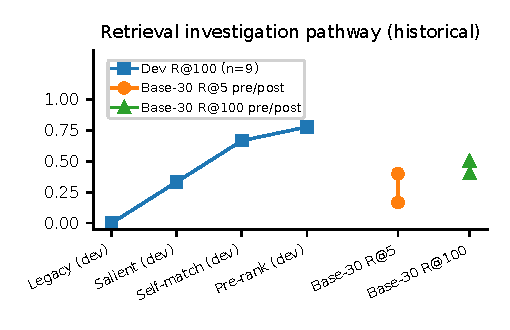
\includegraphics[width=\columnwidth]{figures/fig4_investigation.pdf}
\caption{Retrieval investigation pathway. The nine-case development probe covers
the salient-query and self-match repairs; the separate held-out comparison
($n=30$) covers the move from post-ranking to pre-ranking temporal filtering.
These are two distinct populations, not one learning curve.}
\label{fig:investigation}
\end{figure}

Temporal capacity is not the whole story. Case \texttt{2013\_35} remained absent
despite 79 eligible candidates in its earlier raw top 100, whereas
\texttt{1980\_105} was recovered despite only three eligible candidates and
became a top-five hit. Eligible-pool size and lexical relevance are independent
contributors, and residual lexical mismatch remains the dominant unresolved
cause.

\subsection{Explanation format}

The principal RQ3 evaluation is a blinded exploratory comparison by four
LLM raters (Gemini, Claude Sonnet 4.6, DeepSeek, GPT-5.6 Luna) over 14
paired cases with citations held programmatically constant in shuffled
order: the seven formative pairs plus all seven verified extension cases,
with no cherry-picking. Each rater scored five transparency dimensions on
a 1--5 scale and recorded a forced preference, yielding 112 display-level
ratings and 56 preferences. The structured presentation was preferred in
56/56 evaluations, with mean differences of $+$1.75 (evidence linkage),
$+$1.00 (citation verifiability), $+$2.48 (traceability), $+$2.52
(explanation clarity), and $+$1.98 (transparency/inspectability), for an
overall $+$1.95 (4.66 vs.\ 2.71); see Figure~\ref{fig:explanation}.

\begin{figure}[t]
\centering
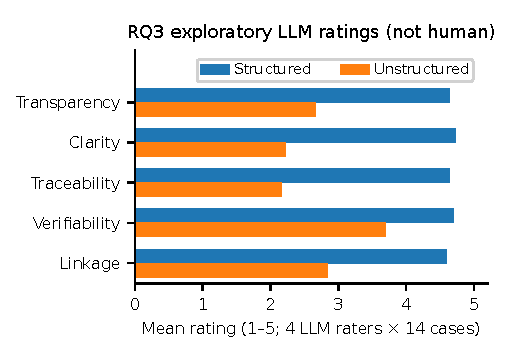
\includegraphics[width=\columnwidth]{figures/fig5_explanation.pdf}
\caption{Blinded LLM-rater means by dimension ($n=14$ cases $\times$ 4
raters). This is exploratory presentation evaluation, not independent
human-subject evidence.}
\label{fig:explanation}
\end{figure}

This is explicitly \emph{not} human evaluation: no independent rater
participated, no significance test was run, and the result establishes
nothing about human preference or legal correctness. Two further cautions
apply. First, the DeepSeek and GPT-5.6 Luna runs produced byte-identical
rating vectors; both are retained and reported separately rather than
merged, so the four-rater unanimity partly reflects duplicated outputs.
Second, the earlier seven-case author self-review (means 4.57 vs.\ 2.71,
4.57 vs.\ 2.29, 4.43 vs.\ 2.86, 4.43 vs.\ 3.00; 7/7 structured) is kept
only as formative, non-independent evidence, superseded by the 14-case
evaluation above. Its most useful output remains negative: generic
uncertainty wording did not adapt to the evidence quality of
\texttt{2013\_35}, indicating uncalibrated caution language that a purely
quantitative evaluation would not have surfaced.

% =====================================================================
\section{Error Analysis}
\label{sec:error}

\subsection{Outcome disagreement}

The analysis is read-only and uses only final frozen outputs; reconstructed E1
and inference-only E2 predictions exactly reproduced their reported metrics
before per-case joining. Across 1{,}503 cases, both models were correct on 684
and both wrong on 368; E1 alone was correct on 238 and E2 alone on 213
(Table~\ref{tab:overlap}). The models therefore make complementary errors, even
though E1 leads in aggregate --- a pattern that suggests ensemble or
disagreement-triggered routing as future work rather than a straightforward
verdict against domain pre-training.

\begin{table}[t]
\caption{Outcome-error overlap by evaluation population. ``E1'' and ``E2'' count cases where only that model was correct.}
\label{tab:overlap}
\centering
\footnotesize
\setlength{\tabcolsep}{4pt}
\begin{tabular}{lrrrr}
\toprule
\textbf{Population} & \textbf{Both} & \textbf{E1} & \textbf{E2} &
\textbf{Neither} \\
\midrule
Full test ($n=1{,}503$)    & 684 & 238 & 213 & 368 \\
Answer key ($n=30$)        & 18  & 3   & 3   & 6 \\
\bottomrule
\end{tabular}
\end{table}

In the evidence-augmented run, E2 was wrong while E3 and E4 were correct for two
cases (\texttt{1974\_36}, \texttt{1984\_136}). E3-correct/E4-wrong and
E3-wrong/E4-correct each occurred in 0/30 cases, because verification changed
neither the selected evidence nor the shared predictor input.

Critically, four cases (\texttt{2008\_1629}, \texttt{1981\_187},
\texttt{1982\_29}, \texttt{1985\_40}) retrieved \emph{and} selected the expected
authority yet still produced an incorrect outcome prediction. Correct authority
recovery does not mechanically imply a correct predicted outcome --- further
support for keeping the two measures apart. No correct prediction was
accompanied by an unsupported citation.

\subsection{Authority-recovery buckets}

Table~\ref{tab:buckets} gives the exhaustive partition. The middle bucket
isolates \emph{selection} failure: the authority was available in the candidate
set but fell outside the five displayed sources, which is addressable by a
better selector under the existing retrieval. The absent bucket requires
improvement upstream, in query representation, lexical matching,
authority-aware ranking, or corpus coverage.

\begin{table}[t]
\caption{Exhaustive authority-recovery partition ($n=30$).}
\label{tab:buckets}
\centering
\footnotesize
\begin{tabular}{p{2.35cm}rp{4.4cm}}
\toprule
\textbf{Outcome} & \textbf{$n$} & \textbf{Cases} \\
\midrule
Retrieved and selected & 12 &
\texttt{2008\_1629}, \texttt{1995\_322}, \texttt{1995\_375},
\texttt{1986\_176}, \texttt{1977\_99}, \texttt{1981\_187},
\texttt{1980\_222}, \texttt{1980\_105}, \texttt{1995\_425},
\texttt{2002\_944}, \texttt{1982\_29}, \texttt{1988\_96} \\
\addlinespace
Retrieved, not selected & 3 &
\texttt{1980\_133} (rank 15), \texttt{1981\_55} (rank 28),
\texttt{1985\_40} (rank 78) \\
\addlinespace
Absent at $k{=}100$ & 15 &
\texttt{1997\_792}, \texttt{1993\_185}, \texttt{1971\_295},
\texttt{1974\_36}, \texttt{1986\_378}, \texttt{1984\_136},
\texttt{2013\_35}, \texttt{1980\_217}, \texttt{1978\_33},
\texttt{1977\_145}, \texttt{1995\_412}, \texttt{1995\_403},
\texttt{1986\_397}, \texttt{1994\_632}, \texttt{1992\_84} \\
\bottomrule
\end{tabular}
\end{table}

\subsection{Worked example: retrieval noise made visible}

Case \texttt{1985\_40} illustrates why extractive presentation aids review. The
facts concern a factory at Atul manufacturing dyes, chemicals, and
pharmaceuticals, and the addition of synthetic organic dyestuffs as item 14D to
the First Schedule of the Central Excise and Salt Act, 1944.

The system displayed five verified citations: \emph{[1984] 3 S.C.R.\ 930},
\emph{[1972] 3 S.C.R.\ 770}, \emph{[1980] 3 S.C.R.\ 1109}, \emph{[1971] 3
S.C.R.\ 506}, and \emph{[1973] 1 S.C.R.\ 822}. The expected authority,
\emph{[1964] 2 S.C.R.\ 888}, was retrieved at rank 78 but not selected.

Inspecting the displayed set, the first concerns excise valuation and the
``related person'' definition for Atul Products, but the second concerns an
industrial dispute at Atul, the third rayon and silk sales tax, and the fifth
cigarette excise duty. The separate authority index and per-evidence blocks made
these apparent subject-matter mismatches visible for review in a way continuous
prose did not. We stress that this is an illustration of navigability, not an
independent annotation that the alternative citations are legally irrelevant.

% =====================================================================
\section{Limitations and Threats to Validity}
\label{sec:limits}

\textbf{Scope.} The study covers English-language Indian Supreme Court judgments
only. It does not evaluate other Indian languages, High Court or lower-court
material, separately versioned statutes, or cross-jurisdictional transfer.

\textbf{Extraction approximation.} Targeted OCR restored 12 of 15 affected PDF
instances; three were excluded and repaired text may retain minor noise. ILDC
provides no gold facts/reasoning boundary, so the deterministic facts rule can
retain some reasoning or omit facts near a boundary.

\textbf{Answer-key size and era concentration.} The evidence evaluation rests on
30 source-verified frozen cases, extended additively to 37 with seven later
verified cases that postdate the original freeze; 13 of the base 30 are from
the 1980s. The combined set is neither large nor era-balanced and should not
be read as representative of the ILDC test set or of
Indian legal research generally. This is the primary constraint on the
generality of the retrieval findings.

\textbf{Single reference authority.} The key records one expected authority per
query, not every relevant source. Authority inconsistency is a reproducible
reference mismatch, not a substantive legal-relevance judgment.

\textbf{Residual recovery gap.} At $k{=}100$, half of the expected authorities
still went unrecovered. Comparing \texttt{2013\_35} against \texttt{1980\_105}
rules out an easy explanation: having enough temporal room for the true
authority to qualify is not, by itself, sufficient for the retriever to
surface it, so the remaining gap has to be attributed to ranking quality
rather than to the eligibility window.

\textbf{Year-level temporal granularity.} ILDC supplies query dates at
year-level precision only. As a result, any candidate sharing a query's year
is excluded rather than risk admitting a source that actually postdates it --
a conservative choice that can discard genuinely eligible evidence. Getting
day-level dates would require manually checking each case against a primary
source, since ILDC's public release does not provide them; the limitation
therefore sits in the dataset, not in how the pipeline parses dates.

\textbf{Bundled verification.} E4 evaluates several integrity checks together
and cannot isolate the causal contribution of any single component.

\textbf{Non-independent explanation review.} The seven-case review is a
non-random author self-review, not independent usability or legal-correctness
evidence. The 14-case LLM comparison that supersedes it is exploratory
presentation evaluation by four model raters, not human-subject evidence;
two of those runs produced identical outputs and are reported separately
rather than merged, so even the unanimous preference partly reflects
duplicated runs.

\textbf{Prototype scale.} Results apply to the frozen implementation and samples
rather than to all users, courts, domains, or changing corpora.

% =====================================================================
\section{Responsible Use and Governance}

The system is designed as a legal-research aid, not an adjudicator or a provider
of legal advice. Although E3 and E4 emit experimental outcome predictions, the
controlled renderer states no legal conclusion beyond supplied evidence, and the
prediction is held in a separate field. A human reviewer remains responsible for
deciding whether retrieved material is relevant, current, authoritative, and
applicable. This allocation follows the concern in \emph{Pooja Ramesh Singh}
that AI may assist legal work but cannot displace human verification and
responsibility \cite{poojasingh2026}.

Risk controls are fail-closed. Evidence with missing dates, same-year ambiguity,
later dates, target identity, or audited duplication is not displayed. A
citation must resolve to exact corpus text and the correct retrieval run;
altered or unsupported material is rejected. Stable source and passage locators
make verification possible without trusting the renderer's prose.

Governance also requires transparent negative results. We preserve the discarded
256-token run, superseded retrieval configurations, the identifier-collision
correction, answer-key replacements, OCR exclusions, and the non-independent
status of the explanation review. Evaluation populations and denominators remain
separate, and alternative citations are not called irrelevant without
annotation.

The source corpora contain public judgments, but public availability does not
remove privacy or misuse concerns. This prototype exposes no end-user search
service and automates no consequential decision. Any deployment would require
access controls, updated source and licensing review, privacy assessment,
independent legal evaluation, monitoring for corpus change, and a defined
correction process.

% =====================================================================
\section{Conclusion and Future Work}

We built and evaluated a provenance-preserving, temporally constrained evidence
workflow for historical Indian Supreme Court research, and kept evidence and
prediction measurements separate throughout.

The principal finding is a dissociation. Every one of 185 displayed citations
across the combined 37 cases passed grounding, provenance, and temporal
verification, with zero unsupported claims across the 37 cases, while 17 of
the 37 independently verified expected authorities were
absent at $k{=}100$. Verification succeeded for what the system displayed; it did not
guarantee that the system found the expected authority. Legal-research systems
therefore benefit from explicit temporal, identity, and provenance controls ---
but those controls must be evaluated \emph{alongside}, never \emph{instead of},
retrieval coverage and human review.

The cross-corpus audit yields a transferable methodological lesson: only 11 of
5{,}391 syntactic identifier matches between ILDC and the eCourts collection
were content-aligned. Identifier equality is a candidate hint requiring content
validation, not evidence of judgment identity.

The supporting results are reported with their limits. On the 1{,}503-case
outcome task the sparse TF--IDF baseline outperformed corrected InLegalBERT
under the frozen settings, a result about this experiment rather than a general
rejection of legal-domain pre-training. Inference-time evidence augmentation
reached 0.6667 accuracy and 0.6032 macro-F1 on the frozen 30-case subset
(0.6486 and 0.6073 on the combined 37), descriptively and under acknowledged
distribution shift. The 14-case structured-presentation comparison is
exploratory LLM-rater evidence, not human preference; the seven-case
self-review beneath it is formative and non-independent.

\textbf{Future work.} The highest-value extension is an era-balanced answer key
of 75--100 cases, large enough to support a paired significance test such as
McNemar's test between retrieval configurations. A blinded review with
independent raters and reported inter-annotator agreement (e.g., Fleiss'
$\kappa$) would replace the formative explanation evidence. A hybrid
dense--sparse retrieval comparison would test whether semantic retrieval closes
the residual lexical misses while retaining the present temporal and provenance
controls, and evidence-sensitive uncertainty language would address the
calibration weakness the review exposed.

% =====================================================================
\section*{Reproducibility}

All configurations, seeds, model revisions, corpus identities, and evaluation
artifacts are frozen and machine-readable. The E2 checkpoint
(\texttt{checkpoint-6318}) is identified by SHA-256
\texttt{924a5bb9\ldots dbdc773}; the evidence-augmented replay produces a stable
output hash. The implementation passes 81 automated tests and the documented
reproducibility checks (14/14 documentation checks and 34/34 freeze-hash
checks in the Week-16 audit), and the evidence-augmented evaluation
replays deterministically from a clean clone. Code and artifacts are available
at \url{https://github.com/0-YuvrajSingh/NyayaTrace}.

% =====================================================================
\begin{thebibliography}{00}

\bibitem{malik2021}
V. Malik, R. Sanjay, S. K. Nigam, K. Ghosh, S. K. Guha, A. Bhattacharya, and
A. Modi, ``ILDC for CJPE: Indian Legal Documents Corpus for Court Judgment
Prediction and Explanation,'' in \emph{Proc.\ 59th Annual Meeting of the
Association for Computational Linguistics (ACL-IJCNLP)}, 2021, pp.\ 4046--4062.

\bibitem{paul2023}
S. Paul, A. Mandal, P. Goyal, and S. Ghosh, ``Pre-trained Language Models for
the Legal Domain: A Case Study on Indian Law,'' in \emph{Proc.\ 19th Int.\
Conf.\ on Artificial Intelligence and Law (ICAIL)}, 2023, pp.\ 187--196.

\bibitem{taxflow2026}
V. R. Karna, R. M. Rajesh, B. S. Babu, S. Neethu, M. Manasa, and V. Harshitha,
``A Hybrid RAG-LLaMA Framework for Scalable and Accurate Interpretation of Legal
Texts,'' \emph{Applied Artificial Intelligence}, vol.\ 40, no.\ 1, art.\
2626097, 2026.

\bibitem{casefacts2026}
A. R. Putta, J. Devasier, and C. Li, ``CaseFacts: A Benchmark for Legal
Fact-Checking and Precedent Retrieval,'' in \emph{Proc.\ 64th Annual Meeting of
the Association for Computational Linguistics}, 2026, pp.\ 17246--17265.

\bibitem{lextime2025}
C. Barale, L. Barrett, V. S. Bajaj, and M. Rovatsos, ``LexTime: A Benchmark for
Temporal Ordering of Legal Events,'' in \emph{Findings of the Association for
Computational Linguistics: EMNLP 2025}, 2025, pp.\ 5220--5236.

\bibitem{poojasingh2026}
Supreme Court of India, \emph{Pooja Ramesh Singh v. Jammu and Kashmir Bank Ltd.\
\& Anr.}, 2026 INSC 668, 2026. Order copy:
\url{https://ibbi.gov.in/uploads/order/8e1ccab8f7f445f81034223c1d0fe7b9.pdf}.

\bibitem{robertson2009}
S. Robertson and H. Zaragoza, ``The Probabilistic Relevance Framework: BM25 and
Beyond,'' \emph{Foundations and Trends in Information Retrieval}, vol.\ 3, no.\
4, pp.\ 333--389, 2009.

\bibitem{smith2007}
R. Smith, ``An Overview of the Tesseract OCR Engine,'' in \emph{Proc.\ 9th Int.\
Conf.\ on Document Analysis and Recognition (ICDAR)}, vol.\ 2, 2007, pp.\
629--633.

\bibitem{coliee2023}
R. Goebel, Y. Kano, M.-Y. Kim, J. Rabelo, K. Satoh, and M. Yoshioka, ``Summary
of the Competition on Legal Information, Extraction/Entailment (COLIEE) 2023,''
in \emph{Proc.\ 19th Int.\ Conf.\ on Artificial Intelligence and Law (ICAIL)},
2023, pp.\ 472--480.

\bibitem{legalbench2023}
N. Guha et al., ``LegalBench: A Collaboratively Built Benchmark for Measuring
Legal Reasoning in Large Language Models,'' in \emph{Advances in Neural
Information Processing Systems 36, Datasets and Benchmarks Track}, 2023.

\bibitem{casehold2021}
L. Zheng, N. Guha, B. R. Anderson, P. Henderson, and D. E. Ho, ``When Does
Pretraining Help? Assessing Self-Supervised Learning for Law and the CaseHOLD
Dataset of 53,000+ Legal Holdings,'' in \emph{Proc.\ 18th Int.\ Conf.\ on
Artificial Intelligence and Law (ICAIL)}, 2021, pp.\ 159--168.

\bibitem{shukla2022}
A. Shukla, P. Bhattacharya, S. Poddar, R. Mukherjee, K. Ghosh, P. Goyal, and
S. Ghosh, ``Legal Case Document Summarization: Extractive and Abstractive
Methods and their Evaluation,'' in \emph{Proc.\ 2nd Conf.\ of the Asia-Pacific
Chapter of the ACL (AACL-IJCNLP)}, 2022, pp.\ 1048--1064.

\bibitem{dahl2024}
M. Dahl, V. Magesh, M. Suzgun, and D. E. Ho, ``Large Legal Fictions: Profiling
Legal Hallucinations in Large Language Models,'' \emph{Journal of Legal
Analysis}, vol.\ 16, no.\ 1, pp.\ 64--93, 2024.

\bibitem{nay2023}
J. J. Nay, ``Large Language Models as Fiduciaries: A Case Study Toward Robustly
Communicating With Artificial Intelligence Through Legal Standards,''
\emph{arXiv preprint arXiv:2301.10095}, 2023.

\bibitem{lewis2020}
P. Lewis et al., ``Retrieval-Augmented Generation for Knowledge-Intensive NLP
Tasks,'' in \emph{Advances in Neural Information Processing Systems 33}, 2020,
pp.\ 9459--9474.

\end{thebibliography}

\end{document}
